%%%%%%%%%%%%%%%%%%%%%%%%%%%%%%%%%%%%%%START PREAMBLE THAT IS THE SAME FOR ALL EXAMPLES
\documentclass{article}

%Required: You must have these
\usepackage{Sweave}
\usepackage{graphicx}
\usepackage{tabularx}
\usepackage{hyperref}
\usepackage{natbib}
\usepackage{pdflscape}
\usepackage{array}
\usepackage{gensymb}
%\usepackage[backend=bibtex]{biblatex}
%Strongly recommended
  %put your figures in one place
%\SweaveOpts{prefix.string=figures/, eps=FALSE} 
%you'll want these for pretty captioning
\usepackage[small]{caption}

\setkeys{Gin}{width=0.8\textwidth}  %make the figs 50 perc textwidth
\setlength{\captionmargin}{30pt}
\setlength{\abovecaptionskip}{10pt}
\setlength{\belowcaptionskip}{10pt}
% manual for caption  http://www.dd.chalmers.se/latex/Docs/PDF/caption.pdf

%Optional: I like to muck with my margins and spacing in ways that LaTeX frowns on
%Here's how to do that
 \topmargin -1.5cm        
 \oddsidemargin -0.04cm   
 \evensidemargin -0.04cm  % same as oddsidemargin but for left-hand pages
 \textwidth 16.59cm
 \textheight 21.94cm 
 %\pagestyle{empty}       % Uncomment if don't want page numbers
 \parskip 7.2pt           % sets spacing between paragraphs
 %\renewcommand{\baselinestretch}{1.5} 	% Uncomment for 1.5 spacing between lines
\parindent 0pt% sets leading space for paragraphs
\usepackage{setspace}
%\doublespacing

%Optional: I like fancy headers
%\usepackage{fancyhdr}
%\pagestyle{fancy}
%\fancyhead[LO]{How do climate change experiments actually change climate}
%\fancyhead[RO]{2016}
 
%%%%%%%%%%%%%%%%%%%%%%%%%%%%%%%%%%%%%%END PREAMBLE THAT IS THE SAME FOR ALL EXAMPLES

%Start of the document
\begin{document}

%\SweaveOpts{concordance=TRUE}

\bibliographystyle{../refs/bibstyles/amnat.bst}% i moved a style file into the ospree git repo. feel free to add whatever style you like and update, lizzie! I don't have besjournals
\title{Shifts in Southern Resident Killer Whale Phenology in the Salish Sea}
\date{\today}
\maketitle
\author{A.K. Ettinger, C. Harvey, J. Samhouri, B. Hanson, C. Emmons, J. Olson, E. Ward}
\maketitle  %put the fancy title on
%%%%%%%%%%%%%%%%%%%%%%%%%%%%%%%%%%%%%%%%%%%%%%%%%%%
\par 
\emph{Target journal(s)}: Global change biology, Journal of Applied Ecology %, Marine Ecology Progress Series, not currently written for a short-form journal but perhaps consider PNAS?
\section* {Introduction}
\par Phenology, or the timing of biological activities such as migration, growth, and reproduction, can have dramatic implications for fitness \citep{lane2012,chuine2010}. Consumer phenology that is out of step with its resource phenology can cause increased mortality \citep{lamaris2018} or reduced reproductive success \citep{post2007}. The critical nature of these ``matches'' or  ``mismatches'' was originally described for fish and zooplankton \citep{hjort1914,cushing1974,cushing1975}, and has received renewed scientific interest as phenological shifts have been increasingly observed in conjunction with recent climate change \citep{durant2007}. 

\par Despite its importance, phenology of many organisms, even those of conservation concern, remains poorly understood and is rarely quantified, especially for marine organisms. A recent meta-analysis found that shifts in marine phenology are at least as dramatic as those observed in terrestrial systems (e.g. −4.4 $\pm$0.7 days per decade) \citep{poloczanska2013}. The abundance of critical resources is more often a focus of natural resource management, yet the timing of resource peaks can be at least as important to consumers \citep{hipfner2008}.
 %JS: I am also thinking that some of the ecological literature on resource pulses could be helpful here, eg Yang et al 2008, 2010
\par Southern resident killer whales (SRKWs, \emph{Orcinus orca}) are a federally endangered population that spends time in the inland waters of Washington State, USA, and British Columbia, Canada.  They have received widespread scientific and public attention in recent years as their numbers have declined\citep[e.g., Seattle Times articles,][]{lusseau2009,larson2018, olson2018}. Insufficient prey availability is believed to be one of the primary threats to this population, along with vessel traffic and pollutants \citep{krahn2007,lusseau2009,hanson2010}. SRKWs differ from many orca whales in that their primary prey are salmon (\emph{Oncorhynchus} species). SRKWs use inland waters to hunt for their prey when they are aggregated and locally highly abundant. Salmon have a distinct seasonality to their migration patterns,  and SRKWs also vary seasonally in their use of inland waters: they travel between summer and winter core areas that can be separated by thousands of kilometers \citep{balcomb1986,krahn2004}. 
\par In recent decades, the abundance and phenology of the favored prey of SRKWs, salmon, has shifted in the western United States \citep{weinheimer2017,reed2011,ford2006,satterthwaite2014}(add Nelson for chinook hatchery release timing), though patterns vary by species and location. We would therefore expect SRKW phenology to have shifted during this time, if prey is a primary driver of their activity in inland waters. If SRKW phenology has not shifted at a rate consistent with phenological shifts in their prey, this mismatch could exacerbate the low prey availability they experience. 
%\par Add a paragraph about monitoring of whales? Quantifying changes in the timing of SRKW activity in inland waters over the pst 40 years is challenging because monitoring effort has increased during this time \citep{olson2018, strebel2014}. 
\par Here, we seek to quantify seasonal variation in SRKW activity and the extent to which these seasonal patterns have shifted over the past four decades.  %CH: I think the overall blueprint is good here; this lays out the objectives and context pretty clearly and will benefit from the additional forthcoming details and perhaps some effort to sharpen the stick a bit and make a clearer case of the urgency faced by the SRKW pop and therefore the importance of this work
Specifically, we ask:
\begin{enumerate}
\item Has the timing of SRKW activity (phenology) shifted in the Salish Sea? 
\item If there have been phenological shifts in SRKW activity, do these shifts coincide with shifts in phenology of their prey (chinook, coho, chum salmon)?
\end{enumerate}

\section* {Methods}
\subsection*{Focal species}:
Add a paragraph here detailing SRKW biology and introducing the three separate pods, as well as the two regions (define them: North= Upper Salish Sea, South = South Puget Sound)

\subsection* {Data}
\par \underline{SRKW}: To quantify SRKW seasonal phenology over time, we used the OrcaMaster Database for Whale Sighting Data (Whale Museum), comprised of data from five main sources, including public sightings networks (e.g., OrcaNetwork), commercial whale watch data, and scientific surveys (e.g., SPOT data from satellite tracking units) \citep{olson2018}. We used data from 1978-2017, because prior to this time there was no dedicated effort to track SRKW presence in the region \citep{olson2018}. We used these sighting data to quantify %first observation day-of-year (DOY, the first date on which one or more pods of SRKWs were observed in a given region) and last observation DOY (the lasst date on which one or more pods of SRKWs were observed) 
detection of SRKWs in the two core areas: the Central Salish Sea, used primarily by SRKWs from May through September, and Puget Sound proper, visited by SRKWs most commonly from September through January \citep{olson2018}. We used these seasonal definitions because they are most aligned with mean SRKW seasonal activity patterns over time (Fig \ref{fig:phenplot}).  We also quantified number of whale days (i.e. days on which whales were observed) within a season and year for each region. 

\par \underline{Salmon}: To quantify SRKW prey phenology over time, we used adult salmon return ('escapement') data for coho, chum, and chinook salmon in Washington state (https://wdfw.wa.gov/fishing/management/hatcheries/escapement), as well as data from the Albion Chinook test fishery on the lower Fraser River at Albion, British Columbia, Canada (https://www.pac.dfo-mpo.gc.ca/fm-gp/fraser/docs/commercial/albionchinook-quinnat-eng.html). Daily or weekly WDFW data are available for 67 streams going back to 1997 and include wild and hatchery counts. We selected sites located close to Puget Sound or the central Salish Sea (i.e.., within XX km) with the greatest available data (i.e., long time series with frequent monitoring), and with relatively large run sizes (range of average counts from trap estimates = 8,640-30,000/134-1,400 for hatchery/wild chum, 11,500/21-621 for hatchery/wild coho, and 550-13,350/36 for hatchery/wild chinook.)

\subsection* {Analysis}
\underline{SRKW}:
\par To identify trends over time in phenology for SRKWs in the Central Salish Sea and in Puget Sound proper, we summarized first-, last-, and mean- observation dates from 1978 through 2017 in each region. %We also compared first and last observation dates across time periods (1978-1997 versus 1998-2018), using t-tests (Fig \ref{fig:boxplot1} and \ref{fig:boxplot2}), because relationships over time did not look linear and linear regression provided poor fit (Fig \ref{fig:reg}). %Could also break this into 4 decade-long time periods- this might capture the recent trend of later arrival to San Juan Island. 
\par  To estimate effects of increased effort (i.e., increased numbers of sightings over time) on trends in phenology, we simulated data sets of whale presence during two seasons equivalent to those in our data set (summer, which was 1 May through 31 Sept, or 153 days, and fall, which was 1 October through 1 Feb, or 123 days). We used whale presence probabilities of 0.85 for the Central Salish Sea and 0.6 for Puget Sound (the means in our data set for each region) and kept it constant over 40 simulated years. We then created an observation data set, in which effort (the number of observations), varied. During the low effort time period (years 1-20), the number of observations had a mean of 15 per year for Puget Sound and 104 per year in the Central Salish Sea (matching the means for these regions from 1978-1997 in the OrcaMaster database).  During the high effort time period (years 21-40 in our simulated data set), the number of annual observations had a mean of 39 for Puget Sound and 133 for the Central Salish Sea (matching those in the OrcaMAster database from 1998-2017). We then calculated first- and last- observations dates for each simulated year. We ran these simulation 100 times and calculated the difference between the low effort and high effort time periods. We compared these to the mean differences first- and last-observation dates across time periods in the OrcaMaster database, for each region, to understand whether observed changes may be due to changes in effort over time, rather than changes in orca activity (Fig \ref{fig:sim}).

\par We quantify pod-specific phenology for J, K, and L pods in the north versus south regions using occupancy models. Occupancy models (MacKenzie et al. 2002) can estimate jointly species presence or abundance and detection probability (the probability to detect at least one individual present at site). We parameterized the model with annual occupancy probabilities (i.e., we did not fit a dynamic model, but a multiseason model (Royle and Kery 2007). The distribution submodel distinguishes true presence or absence of pod,p, (z, a latent state) in marine area i in year t,( add equation here). We assumed zi,t to be a Bernoulli random variable. We modeled detection probability as a function of year and date, with detectability modeled as a semi-parametric, smooth function of date using flexible thin-plate spline regression modelling \citep{strebel2014}. 
\par  We fit separate occupancy models within each region and season, for each pod, and estimated annual first-, last-, and peak detection dates with each model. We defined first-detection date as the first DOY within the season when detection probability exceeded 0.5; last-detection date was the latest DOY within the season when detection probability exceeded 0.5. (Using a threshold probability lowed than 0.5 did not qualitatively alter observed trends, Figure SX.)
\par Add analyses of subsets of data for which effort has not changed so dramatically: Lime Kiln observations for USS; West Seattle observations for PS.
\underline{Salmon}:
\par We used linear regression to identify trends over time in first, median, peak, and last dates of salmon adult migration timing. 

\section*{Results}
\par We found that SRKW phenology has shifted over the past four decades, though not necessarily in a linear fashion. Across the full time span, first-detection dates have gotten earlier by XX days per decade in Puget Sound and have not shifted in the Central Salish Sea (Fig. \ref{fig:shifts}). 
Last-detection dates have gotten later by XX days in Puget Sound and by XX days per decade in the Upper Salish Sea (Fig. \ref{fig:shifts}). Add trends in whale days. %At least some (quantify this?) of these observed shifts are due to increased effort, however (Fig. \ref{fig:sim}).
\par We found that salmon phenology has shifted as well, though the patterns differ across species and regions. In the central Salish Sea, the return timing of wild chinook in the Fraser River has delayed by 8.0 days per decade (75 percent credible intervals: 5-11 days per decade) for first- observations dates from 1980-2018.  Delays in peak return and median return dates are stronger (11.8 and 12.7 days per decade, respectively). Hatchery salmon also showed delays in first and median returns in the central Salish Sea(e.g., chum salmon).
\par In Puget Sound proper where data were available across more streams and the preferred prey of SRKWs are less known, the most common trend for wild and hatchery salmon was a shift toward earlier returns.

\section*{Discussion}
\par The timing of SRKW activity has shifted. Across the full time-series SRKWs, especially J- and L-pods, are arriving earlier in Puget Sound and in the central Salish Sea. SRKWs are spending less time in recent years in the upper Salish Sea. Though the trend across the full time series is earlier first-detection and later last-detection dates, in the last 5-10 years, first-detection dates have gotten later in the upper Salish Sea region.
\par The timing of adult salmon returns has also shifted. Populations in the central Salish Sea are arriving later, whereas many populations in Puget Sound proper, especially hatchery-origin fish, are arriving earlier. 
\par The timing of SRKW activity in central Salish Sea and in Puget Sound proper appears to be shifting in a manner that differs from shifts in salmon timing. This difference may lead to a mismatch between predator and prey that causes additional stress on SRKW populations, since the timing of resource availability can be as important as the amount of the resource \citep[Brianna's work,][]{hipfner2008}
\par Observer effort has shifted over time. Its great that so many people are outside looking for whales! Recommend collecting absence data too. This would allow for more robust analyses of whale distributions. Challenge is increased time/money required for database maintenance with this extra data.

\section*{Conclusion}

\section*{Needs/Questions}

\begin{enumerate}
\item Intro: make a clearer case of the urgency faced by the SRKW pop and therefore the importance of this work
\item Intro: emphasize citizen science a bit more?
\item What other figures would be helpful?
\end{enumerate}

\section* {Figures}

\begin{figure}[p]
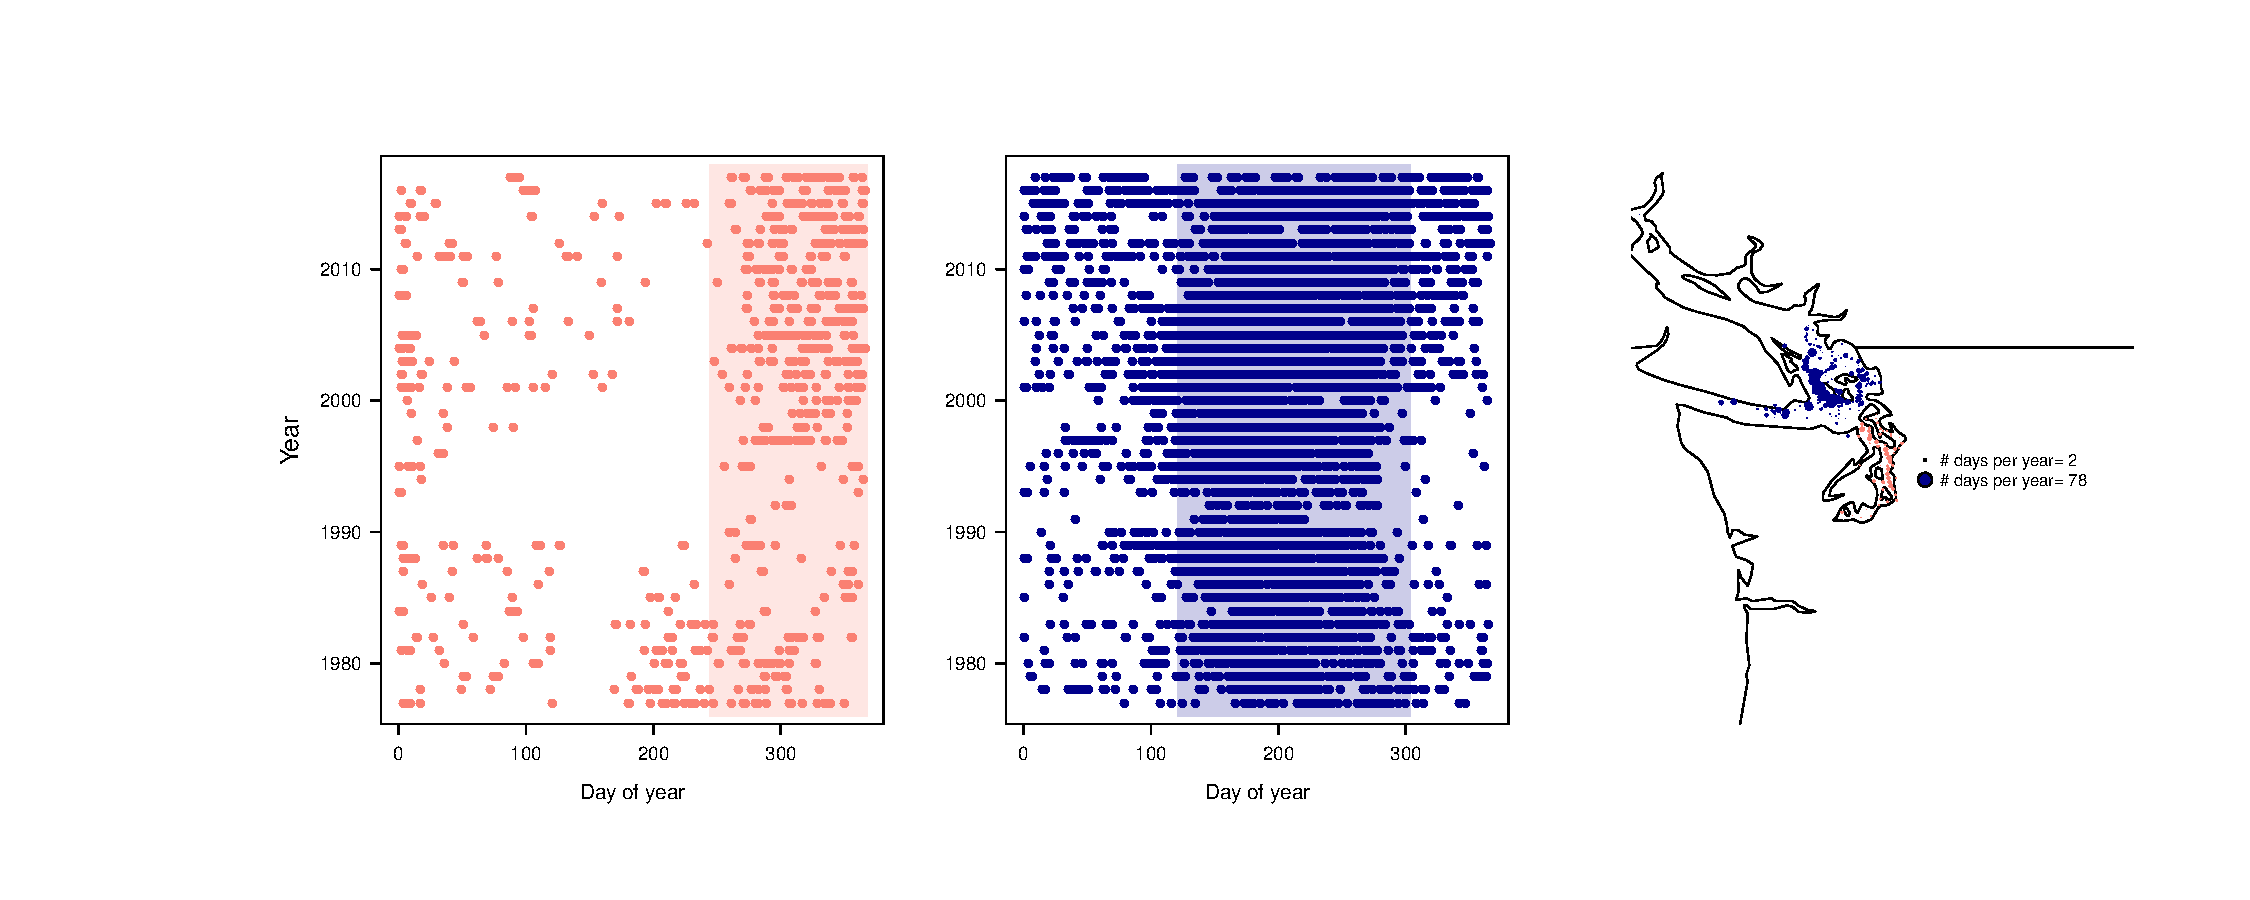
\includegraphics{../analyses/figures/OrcaPhenPlots/srkw_phenmap.pdf} 
\caption{\textbf{Southern resident killer whale activity in the Upper Salish Sea and Puget Sound varies by season}. }
 \label{fig:phenplot}
 \end{figure}
 
%  \begin{figure}[p]
% 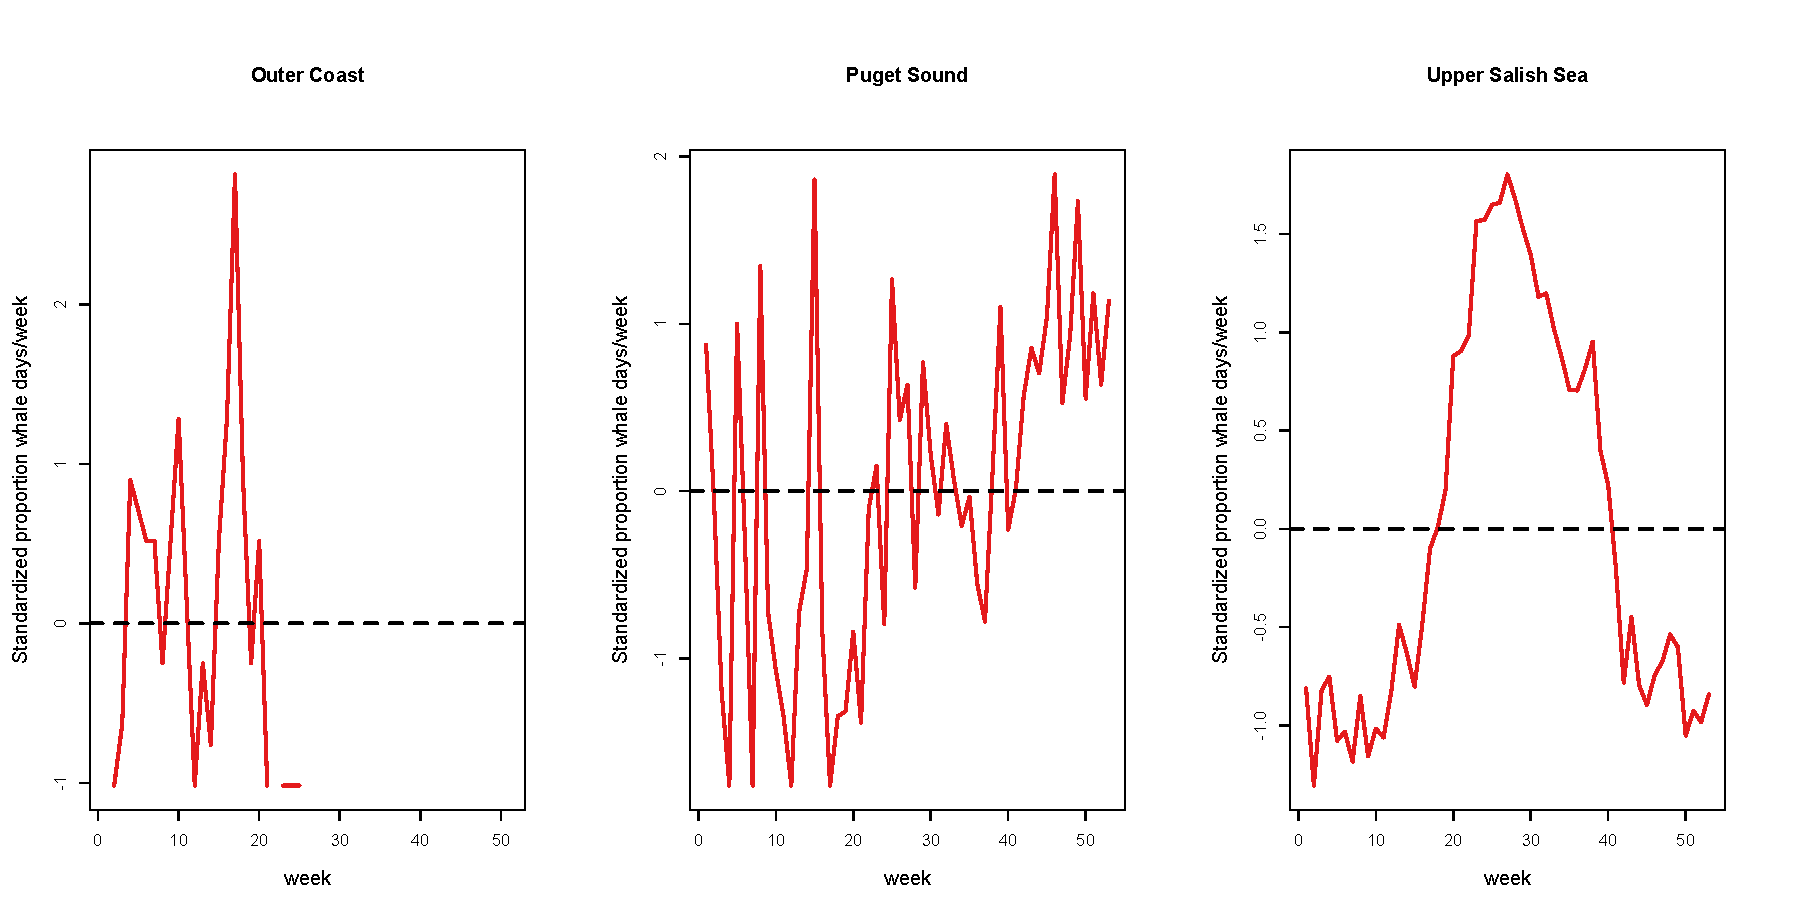
\includegraphics{../analyses/figures/basicplots/propwhdaysperweek_std.pdf} 
% \caption{\textbf{Southern resident killer whale observations, in terms of proportion of days per week that whales were observed, in the Outer Coast, Puget Sound and Upper Salish Sea, varies by season}. Proportions are the mean across all years (1978-2017) and have been standardized by subtracting the mean and dividing by the standard deviation. Thus, the "0" line marks the mean proportion for that region. Weeks range from 1 (i.e., the first week in January) to 52 (i.e., the last week in December).}
%  \label{fig:phenplot1}
%  \end{figure}

%\begin{figure}[p]
%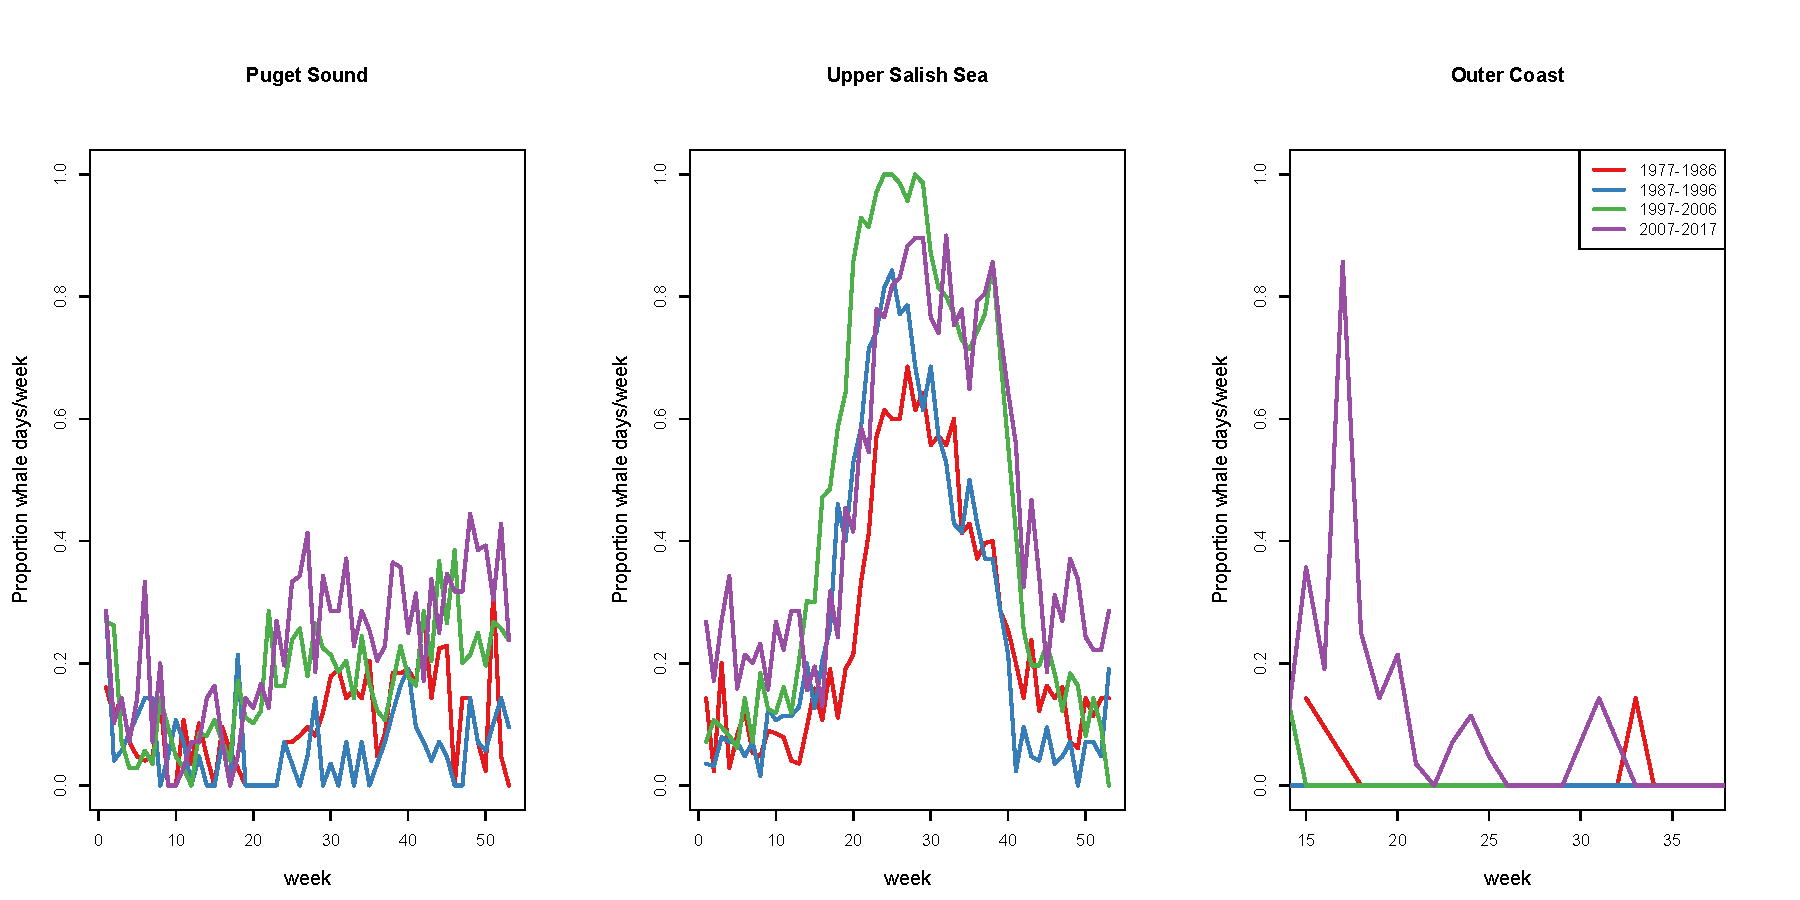
\includegraphics{../analyses/figures/basicplots/propwhdaysperweek.pdf} 
%\caption{\textbf{Southern resident killer whale activity varies by season and region}. Lines show proportion of days per week (1 Jan= week 1) in which whales were observed in the region.}
% \label{fig:phenplot2}
% \end{figure} 
%\begin{figure}[p]
%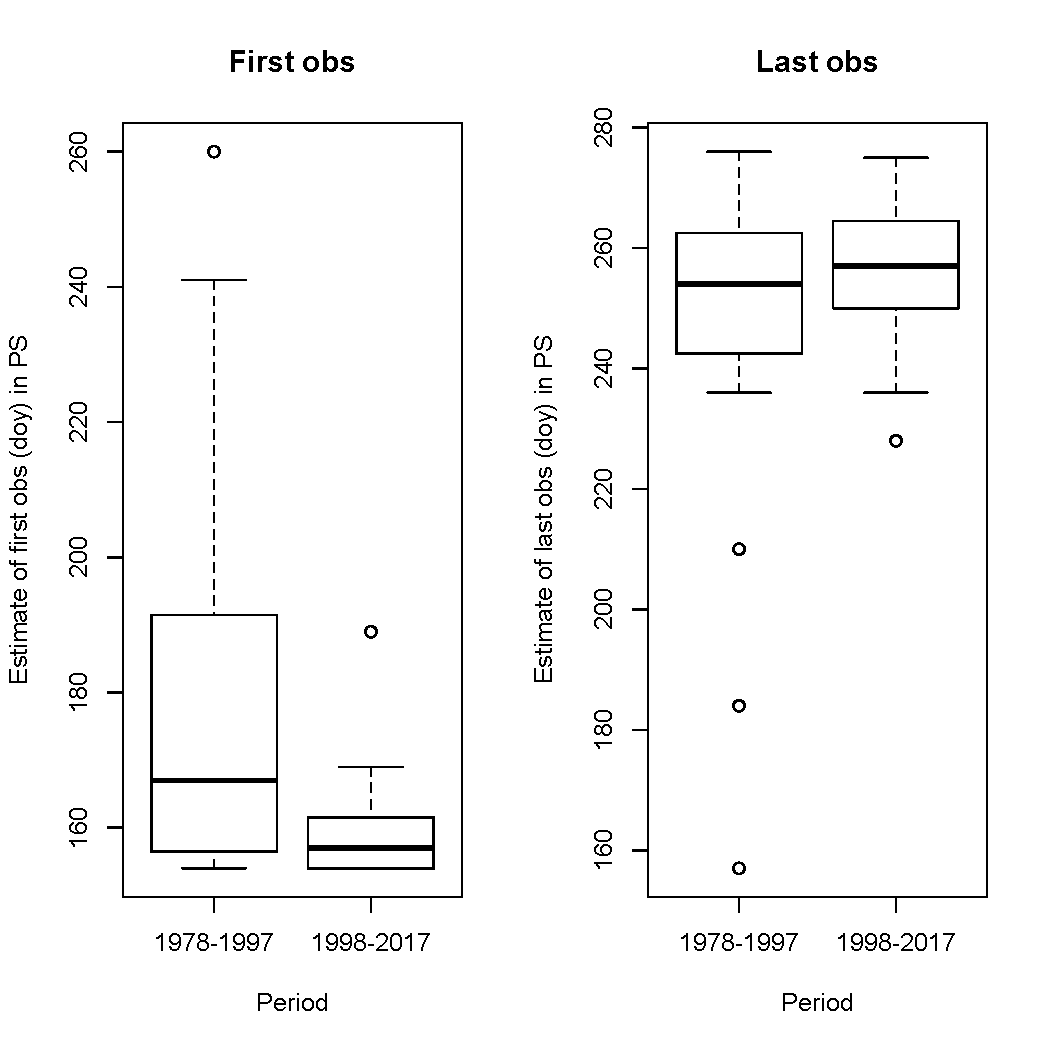
\includegraphics{../analyses/orcaphen/figures/boxplots_1978_2017_ps.pdf} 
%\caption{\textbf{Change in in first and last observation %dates of SRKW in Puget Sound.} }
% \label{fig:boxplot1}
% \end{figure}
% \begin{figure}[p]
%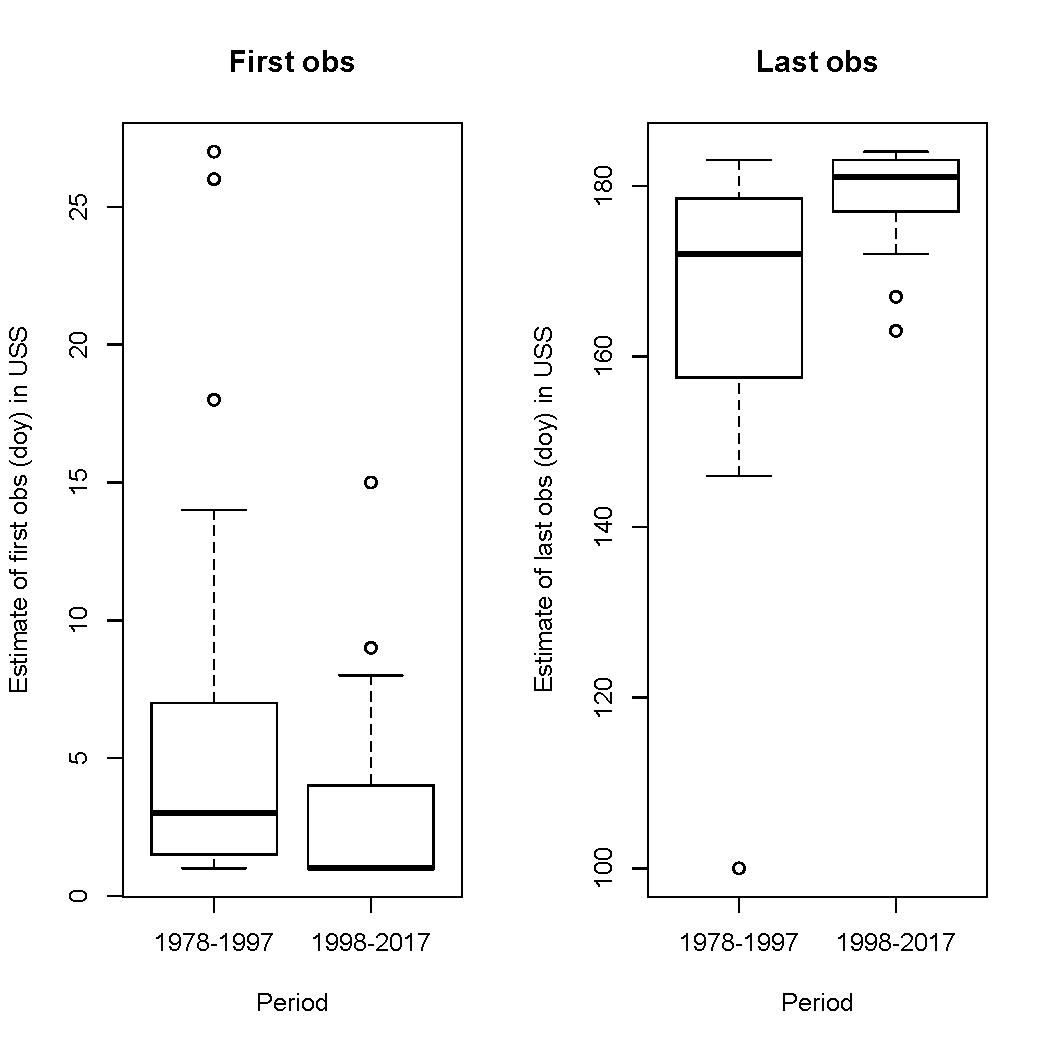
\includegraphics{../analyses/orcaphen/figures/boxplots_1978_2017_uss.pdf} 
%\caption{\textbf{Change in in first and last observation dates of SRKW in the Upper Salish Sea.} }
% \label{fig:boxplot2}
% \end{figure}
 
%\begin{figure}[p]
%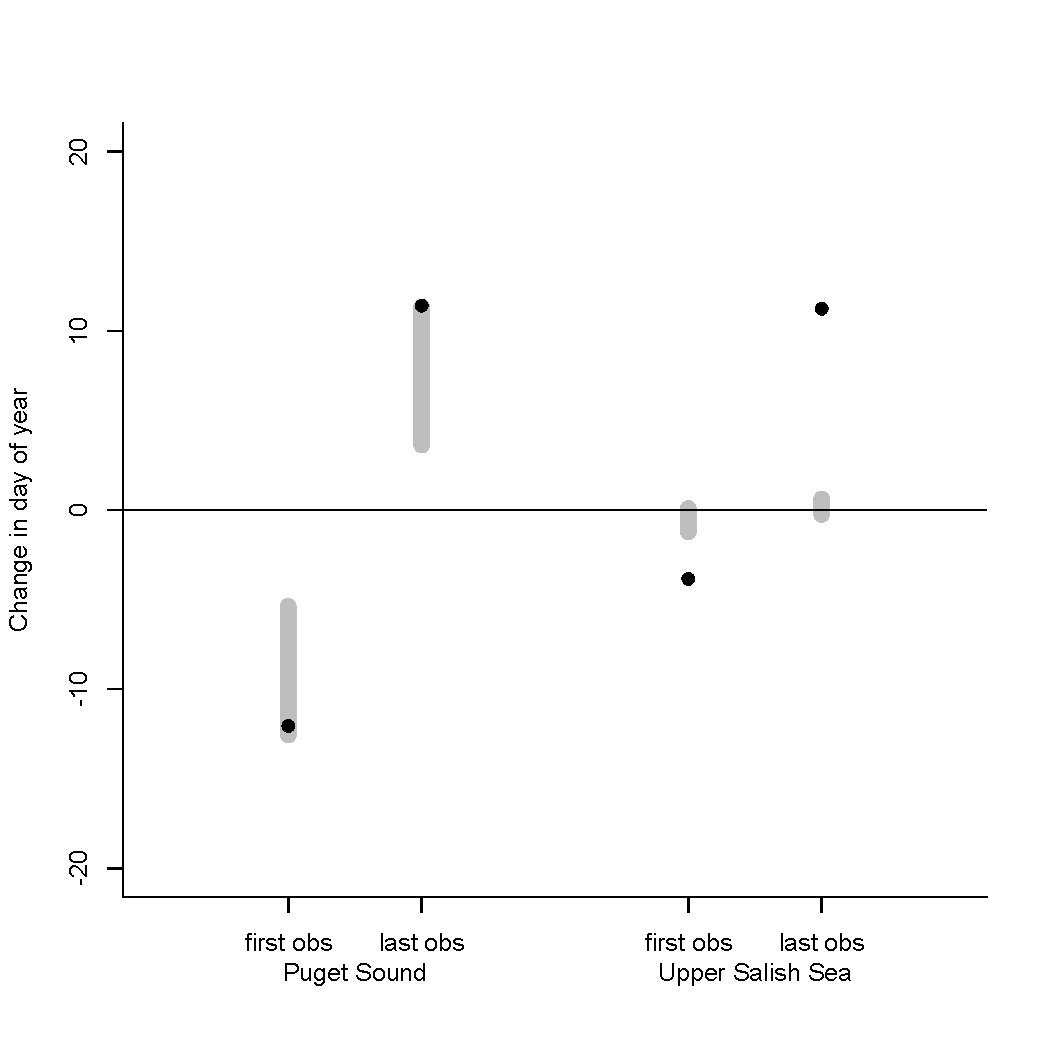
\includegraphics{../analyses/orcaphen/figures/simvdata_1978_2017.pdf} 
%\caption{\textbf{Change in first and last observation dates in Puget Sound and the Upper Salish Sea.} Observed changes (black dots) are compared with expected changes due to shifts in effort alone (gray lines show 90 quantiles of from a simulated data set resulting from shifts in effort, with the probability of SRKW presence was kept constant across time).}
% \label{fig:sim}
% \end{figure}
 

%  \begin{figure}[p]
%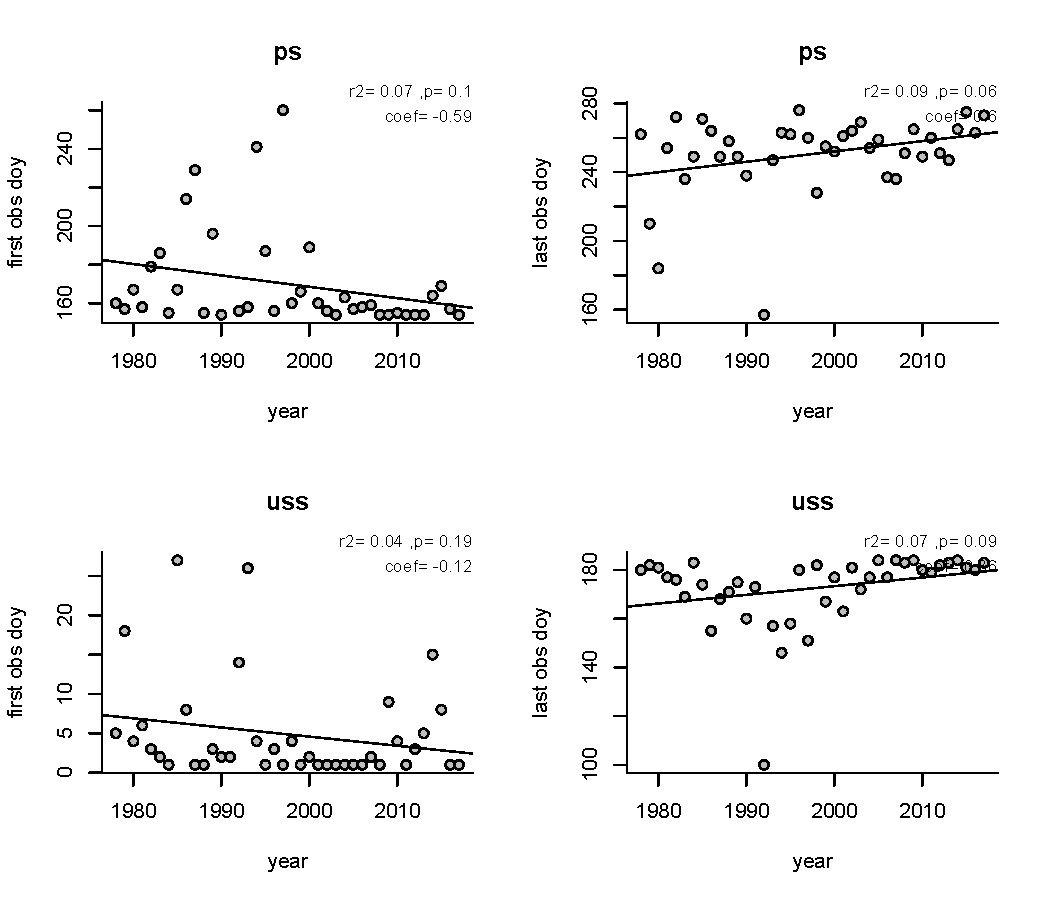
\includegraphics{../analyses/orcaphen/figures/linreg_1978_2017.pdf} 
%\caption{\textbf{Time series and linear regression of first and last observation dates of all SRKW pods.} observed in Puget Sound (upper panels) versus the upper Salish Sea (lower panels). Explanatory power of pod-specific models is generally greater (e.g. Fig. \ref{fig:J}, Fig. \ref{fig:K})}
% \label{fig:reg}
% \end{figure}
 
%\begin{figure}[p]
%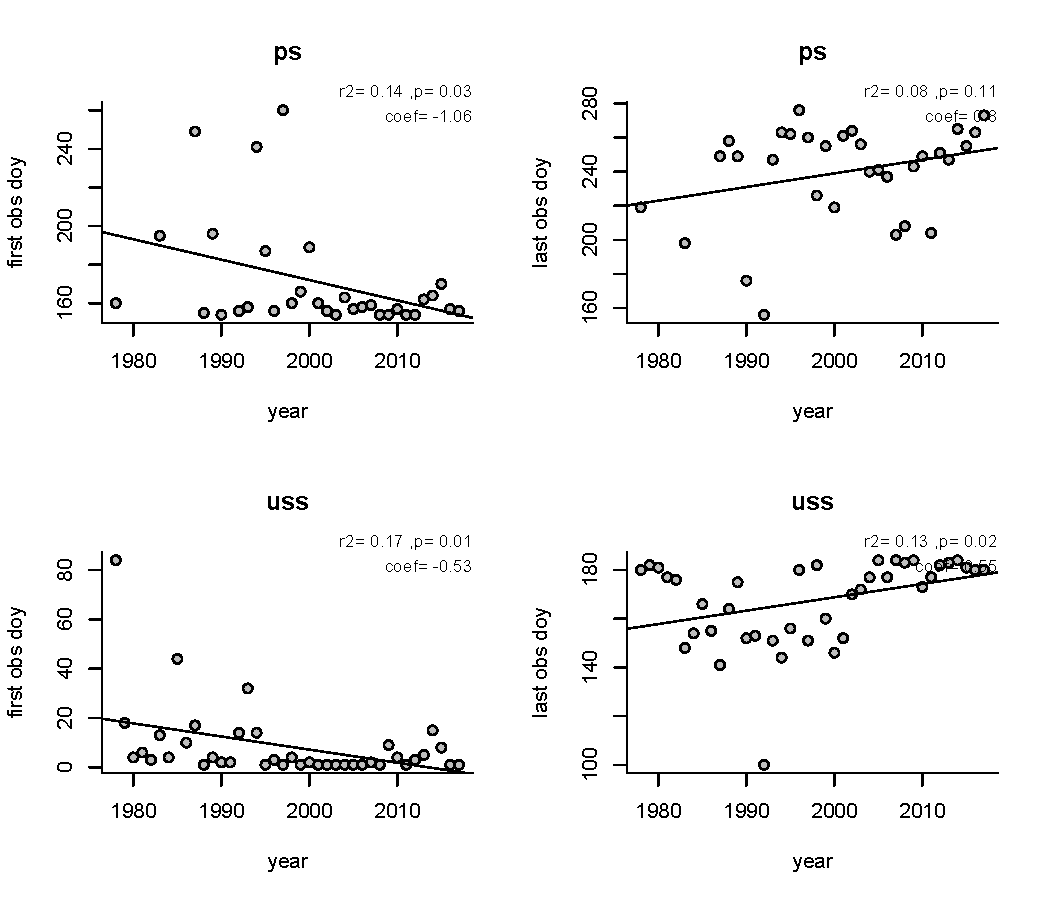
\includegraphics{../analyses/orcaphen/figures/J_linreg_1978_2017.pdf} 
%\caption{\textbf{Time series and linear regression of first and last observation dates of J pod.}- not with occupancy models}
% \label{fig:J}
% \end{figure}
%\begin{figure}[p]
%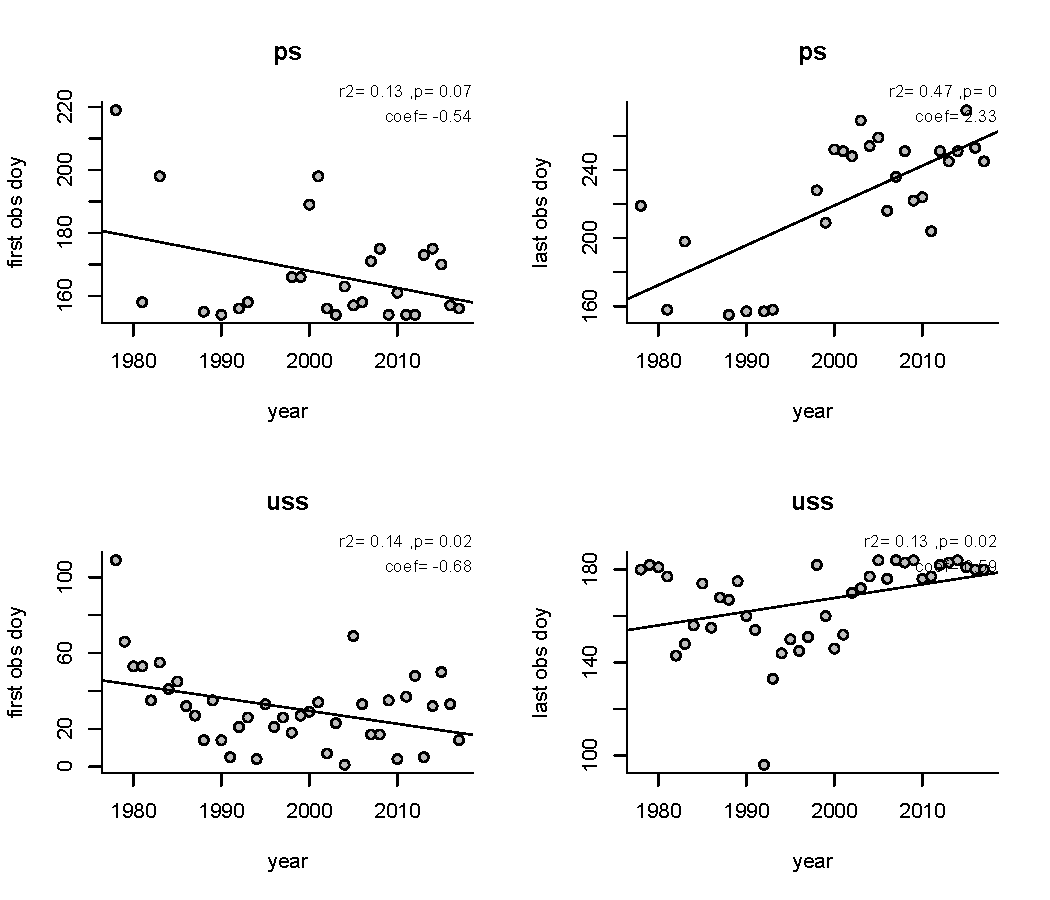
\includegraphics{../analyses/orcaphen/figures/K_linreg_1978_2017.pdf} 
%\caption{\textbf{Time series and linear regression of first and last observation dates of K pod.}- not with occupancy models}
% \label{fig:K}
% \end{figure}
 
\begin{figure}[p]
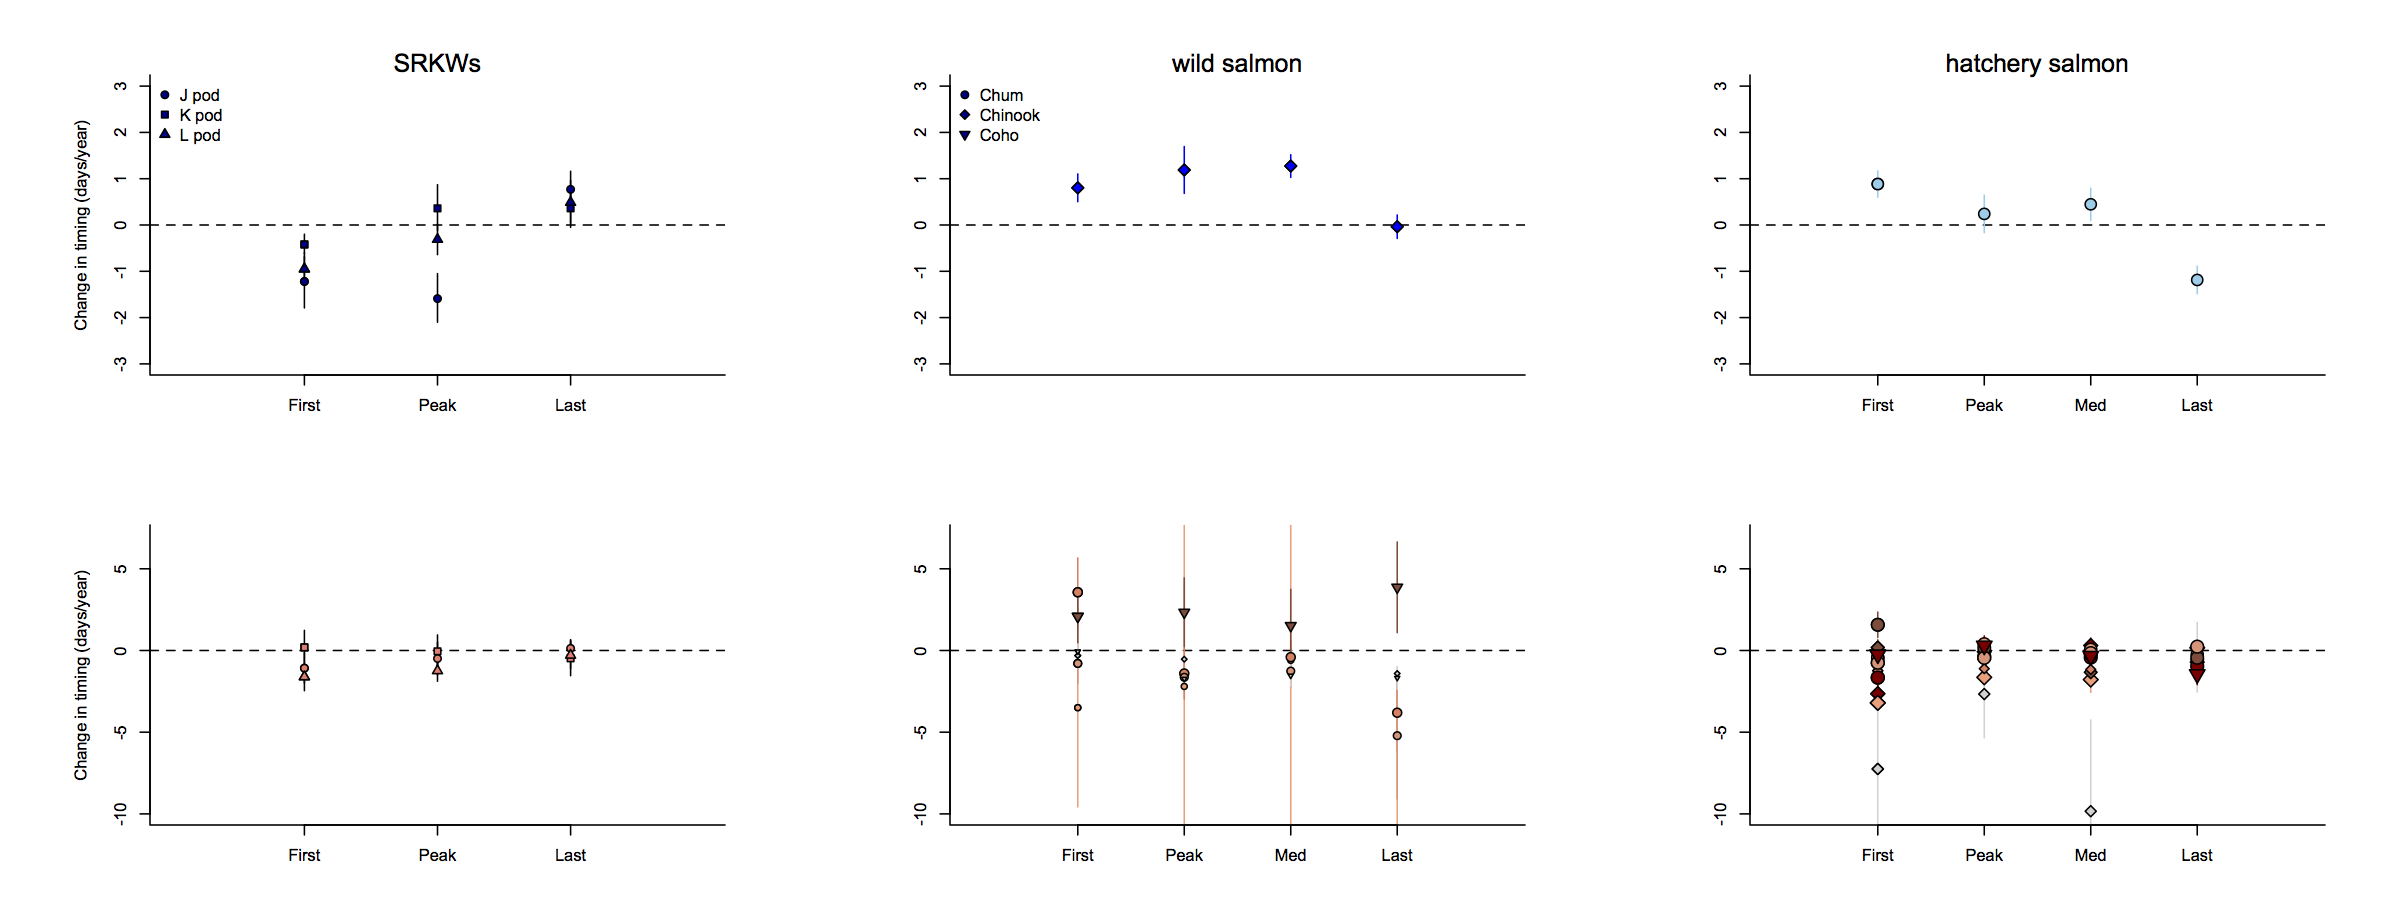
\includegraphics{../analyses/figures/srkw_salmon_shifts_lm.png} 
\caption{\textbf{Trends in first-, peak-, and last- observation dates for SRKWs and their prey.}}
 \label{fig:shifts}
 \end{figure}

%\begin{figure}[p]
%\includegraphics{../analyses/figures/wdfw_returns/salmonshiftsmapwasize.pdf} 
%\caption{\textbf{Salmon return timing is shifting}, though patterns vary by stream and species.}
% \label{fig:salmon}
% \end{figure}

\bibliography{../refs/noaalib.bib}
\end{document}
